\section{Implementation}
\label{sec:implementation}


\begin{figure}[htbp]
	\centering
	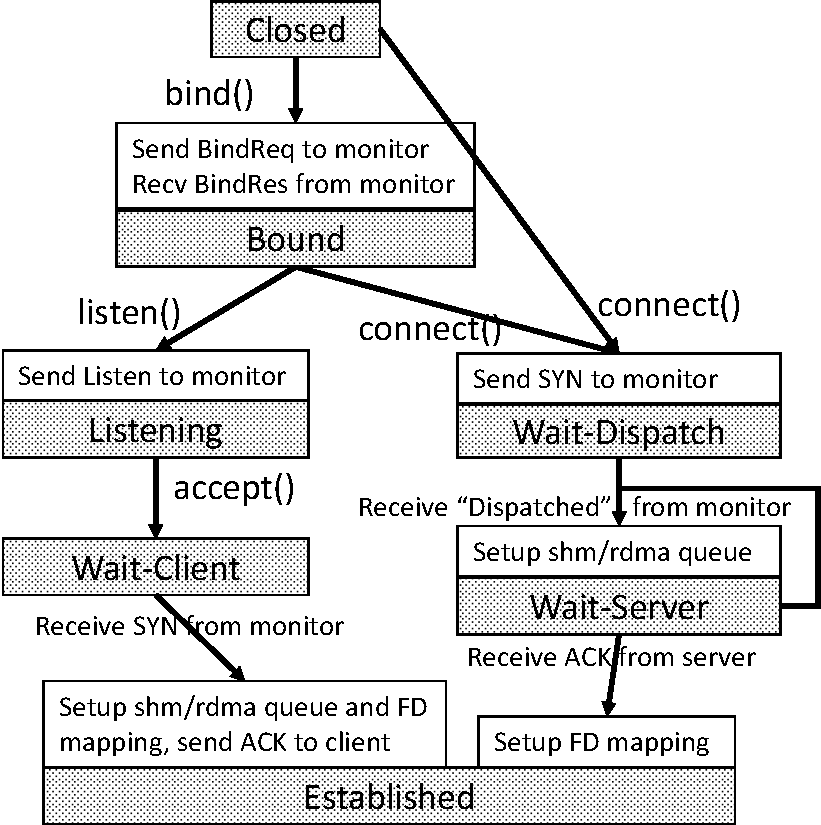
\includegraphics[width=0.3\textwidth]{images/conn-setup-new}
	\vspace{-5pt}
	\caption{State machine of connection creation.}
	\vspace{-10pt}
	\label{fig:conn-setup}
\end{figure}
\begin{figure}[htbp]
	\centering
	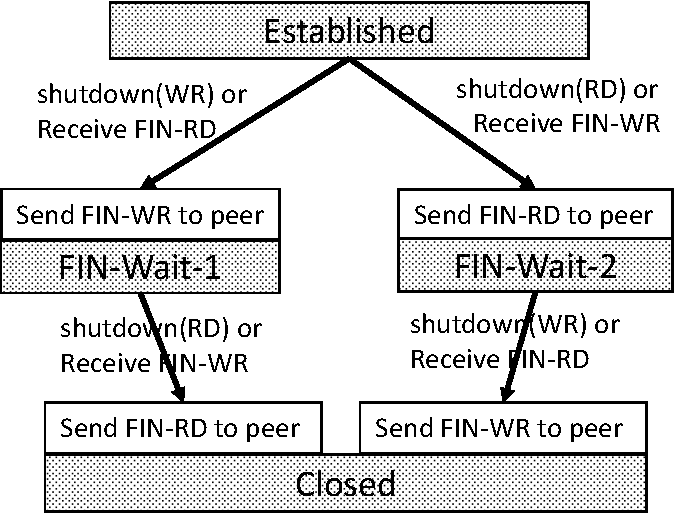
\includegraphics[width=0.25\textwidth]{images/conn-close-new}
	\vspace{-5pt}
	\caption{State machine of connection close.}
	\label{fig:conn-close}
	\vspace{-15pt}
\end{figure}

For implementation, \libipc is divided to two parts: monitor and userspace library. Both parts are implemented in $\approx$5000 lines of C/C++ code. %We take advantage of C++ templates for different types of queues in our design.


\parab{Connection creation.}
in Figure~\ref{fig:conn-setup}...

During initialization, \libipc{} connects to the monitor in local host via TCP socket (called \emph{bootstrap socket}) and establishes a shared memory queue between them.
Since then, communication between the application and monitor go through the shared memory queue.

When an application creates a connection, it sends the request to monitor.
The monitor dispatches the new connection to a listening process (note that there may be many operations).

(a TCP socket on localhost or a local container in overlay network, or a UNIX socket), it connects 


Client application sends a request to client monitor.
Monitor translates IP addresses (NAT), and forward the request to server application:
If the server application is in the same host, forward the command to server application.
If the client and server applications are in different hosts:
If client monitor has connected to server monitor, forward the request to server monitor.
Otherwise, the client monitor and server monitor establish an RDMA connection (details in next slide).
The server monitor forwards the command to server application.
If the client application has not connected to the server application, the server monitor helps the client and server establish a direct connection.
For intra-host, the monitor allocates a shared memory and sends the shared memory key to both client and server applications.
For inter-host, the client and server monitors proxy information between client and server applications during RDMA setup.
The server application sends a response to client application containing FD mapping. The server application can start sending data immediately after sending the response.
When the client application receives the response, it can start sending data.


\parab{Connection close.} in Figure~\ref{fig:conn-close}...

\parab{Detect whether the peer supports \sys{}.}
Goals: Both client and server can detect whether the peer supports SocksDirect. Use kernel TCP when the peer does not support SocksDirect. No change to kernel.
Server monitor opens a raw socket with libpcap to capture SYN packets to listening ports.
Client monitor opens a raw socket with libpcap to send TCP SYN with a special TCP option, then wait for SYN+ACK response.
If server monitor receives a TCP SYN with special option, respond SYN+ACK with special option and begin SocksDirect establishment.
If client monitor receives a TCP SYN+ACK with special option, the peer supports SocksDirect.
To avoid the kernel TCP stack from sending RST packets, install firewall rules to block incoming SYN and outgoing RST.
If the peer does not support SocksDirect:
The monitor creates a kernel TCP connection using TCP restore functionality.
If the application is able to share network namespace with the monitor, send the restored TCP connection to the application via “sendmsg”. Then the application can use the kernel TCP socket.
Otherwise, the monitor proxies messages between the application and kernel TCP socket.


\textbf{Above is draft.}

\parab{\texttt{Socket}.}
As shown in Figure~\ref{fig:socket-pseudo-code}, to create a socket connection, an application first calls \texttt{socket} to get a \textit{file descriptor} (FD). 
%Although Linux globally allocates the lowest available file descriptor, this property is rarely used~\cite{han2012megapipe,huang2017high}. We relax the semantics and maintains an FD table in each process. 
We maintains an FD table for each process. Upon allocation, \libipc{} finds an idle FD from the table or doubles the table size if none available. 
%The table is a vector of socket information with an allocation pointer, indexed by FD. Upon allocation, \libipc{} linearly moves the allocation pointer and finds the first idle FD. When the vector is more than half full, its size is doubled. This allows amortized O(1) allocation and O(1) lookup and deletion.
For multi-thread applications, since the FD namespace is shared, we partition the FD namespace to multiple ranges and each thread allocates FD in its range.
%Because per-FD information is local to a process, APIs on socket options are also local.
Because applications still need to access FDs in the kernel (\textit{e.g.} files and devices), we partition the FD space. The kernel assigns FD from zero up to $2^{30}-1$, while \libipc assigns FD from $2^{31}-1$ down to $2^{30}$.

\parab{\texttt{Bind} and \texttt{listen}.}
A \emph{server} process \texttt{bind}s a socket and needs to detect IP and port conflict. In this case, \texttt{bind} is non-partitionable and goes to the monitor. The monitor also listens on the IP and port in a user-space TCP/IP stack (\textit{e.g.} mTCP~\cite{jeong2014mtcp}, LibVMA~\cite{libvma} or Seastar~\cite{seastar}) to receive connections from other hosts.

A \emph{client} process typically \texttt{bind}s without specifying IP and port, so we need to allocate a unique IP and port for it. For scalability, we partition the loopback IP address space (127.0.0.0/8) and each process allocates IP and port in its range.

\parab{\texttt{Connect} and \texttt{accept}.}
When a client process connects to a server process on the same host, it sends a \textit{connect request} to the monitor via shared memory queue. When the server process is on another host, it creates a \textit{bootstrap TCP socket} with a special option via the user-space TCP/IP stack. If the server host supports the option, it is a \sys host and its monitor establishes an RDMA connection to the client to speedup later communications. Otherwise, the client process keeps using the bootstrap TCP socket for compatibility.

On a server host, the monitor distributes connect requests to server processes in a round-robin order, and a \textit{backlog} is maintained in each process. If the client is TCP only, the monitor proxies messages between the server process and the user-space TCP/IP stack. If the client is intra-server or RDMA capable, and it is the first time for the client and server processes to communicate, the monitor creates an inter-process queue for the process pair and sends the credentials to both processes via bootstrap sockets. After a server process \texttt{accept}s a connection in the backlog, it sends a message to the client via inter-process queue to create an FD mapping, then the socket is ready for data transmission. As Figure~\ref{fig:conn-setup} shows, connection creation takes three inter-process delays.

Distributing connection to listeners may lead to starvation when a listener does not \texttt{accept} new connections. We devise a \textit{work stealing} approach. When a listener \texttt{accept}s from empty backlog, it requests the monitor to steal from others' backlog. To avoid polling empty backlogs, each listener notifies the monitor when its backlog becomes empty. To avoid contention between a listener and monitor, the monitor sends a request to the listener rather than stealing from the backlog directly.

%\subsubsection{Connection Close}

\parab{\texttt{Close} and \texttt{shutdown}.}
Connection close is a peer-to-peer operation because only the peer process needs to be notified. If FD is deleted immediately after \texttt{close}, a new connection may reuse the FD while the peer process might not yet have received the close event thus sends data to the wrong connection. To avoid this, we require a handshake between peers.
Because socket is bidirectional, \texttt{close} is equivalent to \texttt{shutdown} on both send and receive directions.
When application shuts down one direction of a connection, it sends a \textit{shutdown message} to the peer. The peer responds with a shutdown message. A process deletes an FD when it receives shutdown messages in both directions.

%In order to achieve high scalability, we separate scalable operations to different processes. To avoid the overhead of contention, \libipc enable the file descriptor allocation by individual process and when a connection is setup, the other peer of the connection gets notified of the file descriptor number by message passing. Since we treat different threads in one process as different processes, we allocate file descriptor of different ranges to each of them to avoid collision. Since file descriptor is managed separately by each process, it is possible that a file descriptor is reused after the connection is closed. Our solution is that resources of a file descriptor is not released until an ACK is received for the close operation.

%Generally, each process in our design is treated as an endpoint in the network. Figure \ref{fig:conn-setup-close} shows the process of connection setup and close. When \textit{socket} is called, the process itself allocate per fd resources. When \textit{listen} is called, monitor is notified of port occupation. During the \textit{connect} operation, monitor first chooses one of the processes listen on this port then coordinates the creation of the shared memory between the two processes and notifies each other of the new connection. When \textit{close} happens, both of the endpoint notify each other and monitor is responsible to destroy the shared memory between them. 





%\subsection{Seamless system call hook}
%\label{subsec:syscall-hook}

%\parab{LD\_PRELOAD to intercept Linux APIs.}
%\libipc uses \textit{LD\_PRELOAD} environment variable in Linux to load a shared library and intercept the system call wrappers of GNU libc.

%\parab{Multiplex FD between kernel and \libipc{}.}
%Taking the idea of MegaPipe~\cite{han2012megapipe} and LOS~\cite{huang2017high}, we partition the FD space between \libipc and Linux kernel. Linux assigns FD from zero to $2^{30}-1$, while \libipc assigns FD from $2^{31}-1$ down to $2^{30}$.

%\parab{Multiplex events between kernel and \libipc{}.}
%The FD set of \texttt{epoll} may include both sockets and other \textit{kernel FDs} handled by Linux kernel.
%LOS~\cite{huang2017high} periodically invokes non-blocking \texttt{epoll\_wait} syscall with kernel FDs, which leads to a trade-off between delay and CPU overhead. Differently,
%\libipc{} creates a per-process \textit{epoll thread} which runs an infinite loop of blocking \texttt{epoll\_wait} syscall with kernel FDs. Whenever epoll thread receives a kernel event, it broadcasts the event to application threads via shared memory queues. \texttt{Epoll\_wait} in \libipc{} will return such kernel events in addition to socket events. Note that Linux allows an event to be received by multiple threads sharing the FD.

%\textbf{Accelerate access to local storage.}
%Use SPDK and user-mode file system (cite). How to multiplex processes in accessing a file system? (1) directory and metadata go to monitor, (2) read/write within allocated area of a file: process self, (3) append or read/write outside allocated area: handled by master process of a shared file. Monitor pre-allocate free blocks to processes (batch allocation and free).
